
\newpage
\section{Cahn Hilliard equation }%
\label{sec:cahn_hilliard_equation}


% \begin{itemize}
%     \item Explain the full discretization scheme including Follow \cite{feng2007fully}
%     \item CutFEMCIP for spatial discretization
%     \item implicit Euler for temporal discretization
%     \item linearization of nonlinearity (IMEX)
% \end{itemize}


\subsection{The linear Cahn-Hilliard}%

We will consider linear Cahn Hilliard problem. Let $ u( x,0) =  u_{0}$ then is the formulations

\begin{equation}
\label{eq:ch_exact}
    \begin{split}
        \partial _{t} u  + \varepsilon \Delta^2   u -   & =  g_{0}(x)  \quad \text{in} \Omega \\
        \partial _{n} u & =  g_{1}(x)  \quad \text{ on } \Gamma \\
         \partial _{n} \Delta u & = g_{2}(x)  \quad \text{ on } \Gamma  \\
    \end{split}
\end{equation}



We can see that the simplest weak formulation for $u,v \in H^{4}( \Omega ) $ is on the form,
\[
( \partial _{t}u, v )_{\Omega }  - \varepsilon ( \Delta^2 u, v)_{\Omega } = ( h,v)_{\Omega }   \\
\]
We can easily observe that the biharmonic equation is a term of this equation. Combining the theory from \ref{sec:cutcip_biharmonic_problem} and can we see that the Laplace formulation



\subsection{The general Cahn-Hilliard problem}%
\label{sub:the_problem}

Recall the strong form Cahn-Hilliard equation. Let $ u( x,0) =  u_{0}$ then is the dynamics on the form,


\begin{subequations}
    \label{eq:ch_gen}
    \begin{align}
    \label{eq:ch_gen:a}
        \partial _{t} u + \Delta  \left(  \varepsilon  \Delta u - \frac{1}{\varepsilon }f( u) \right)   &= g_{0}( x)   \quad \text{ in } \Omega  \\
        \partial _{n} u &= g_{1}( x)  \quad \text{ on } \Gamma  \\
        \partial _{n}    \Delta u   &= g_{2}(x)  \quad \text{ on } \Gamma
    \end{align}
\end{subequations}
where we defined $f( u) = F'( u) =u( u^2 -1)  $ for $F( u) = \frac{1}{4}( u^{2} - 1)^{2} $ and the domain $\Omega \subset \mathbb{R} ^{d} $  for $d = 2,3$. In contrast to the standard version presented in the introduction \eqref{eq:strongch}, is this version
generalized to also holds for for functions $g_{0},g_{1},g_{2}: \Omega \to\mathbb{R}   $. While the standard version may be physical correct, this version creates flexibility so we can easily construct manufactured solution on complex domains.

    Designing a manufactured solution using $g_{0}( \cdot ) $ may be temping with the formulation \eqref{eq:ch_gen:a}. However, observe that expanding the Laplacian we get,
    \begin{equation}
    \begin{split}
        \Delta  \left(  \varepsilon  \Delta u - \frac{1}{\varepsilon }f( u) \right) & = \varepsilon \Delta^2 u - \frac{1}{\varepsilon } \Delta f( u) \\
                                                                                    &= \varepsilon \Delta ^2 u  - \frac{3}{\varepsilon }( 2u \| \nabla u \|_{ 2 }^{ 2 } + u^{2}  \Delta u )   \\
    \end{split}
    \end{equation}
Here we applied the chain rule twice and inserted the derivatives.
\begin{equation}
    \label{eq:nonlinear_laplace}
    \begin{split}
\Delta f( u)  &= \nabla \cdot \nabla f( u)  = \nabla \cdot  \left[ f' ( u) \partial _{x_{1}}u, \ldots, f' ( u) \partial _{x_{d}}u \right] ^{T} \\
& =  f'' ( u)( ( \partial _{x_{1}}u )^{2} + \ldots +( \partial _{x_{d}}u )^{2} ) +  f' ( u)( \partial _{x_{1} x_{1}}u + \ldots +   \partial _{x_{d} x_{d}}u ) \\
&=  f'' ( u) \| \nabla u \|_{ 2 }^{ 2 } + f' ( u)  \Delta u  = 6u \| \nabla u \|_{ 2 }^{ 2 } + 3u^{2}  \Delta u
    \end{split}
\end{equation}

\subsection{ Numerical scheme for the Cahn Hilliard Equation}%
\label{sub:writing_the_cahn_hilliard_equation_of_weak_form}

Our goal is to write the Cahn Hilliard equation on weak form.
Assume that $\Omega  \subset \mathbb{R} ^{d}$ with a $\Gamma $ in $C^2$.
 Let $u \in  H^{4}( \Omega ) $ and $v \in V_{h} $.
Now, expanding the first Laplace operator from a weak point of view is it clear that
\[
 ( \Delta ( \varepsilon  \Delta u - \frac{1}{\varepsilon } f( u) ) ,v )_{\Omega } = \varepsilon ( \Delta^{2} u ,v )_{\Omega } - \frac{1}{\varepsilon } ( \Delta f( u)  ,v )_{\Omega }.
\]
Hence, this makes it natural to associate the biharmonic $( \Delta ^2 u,v)_{\Omega } $ with bilinear forms $A_{h}( \cdot ,\cdot ) $ , however, in this section will we only consider the Laplace
variant $a^{L}( \cdot ,\cdot ) $.

We will now find seek to find a bilinear form of the nonlinear term,
\begin{lemma}[Semi-linear form]
    Let $u \in H^4( \Omega ) $ be solution to \eqref{eq:ch_gen} and $v_{h} \in V_{h}$ the test function.
Then can we rewrite the nonlinear term into the corresponding semi-linear form $c_{h}( \cdot ,\cdot )  $ for the nonlinear term $( -\Delta f( u) , v_{h})_{\Omega }$ into two consistent formulations.
\begin{enumerate}[label=\arabic*)]
    \item  $c^{}_{h} ( u,v_{h})  = ( f' ( u) \nabla u, v_{h} )_{\Omega }  - ( f'( u)  g_{1}   ,  v_{h})_{\Gamma }$
    \item
        $c^{}_{h} ( u,v_{h})  = -( f( u), \Delta v_{h} )_{\Omega }+  ( f( u) , \jump{ \partial _{n}v_{h} }  )_{\mathcal{F} _{h}^{int}} + ( f(u), \partial _{n} v_{h})_{\Gamma  }  - ( f'( u)  g_{1}   ,  v_{h})_{\Gamma }$
\end{enumerate}
% \begin{remark}
%     Be aware that the both formulations are consistent and if we replace $u \in H^{4}( \Omega ) $ with  $u_{h} \in  V_{h}$ we have two different discrete formulations.
% \end{remark}

\end{lemma}
% \todo[inline]{ I criticize \cite[ Remark 4.1d]{feng2007fully} which says that says that finding this weak form is not possible for conforming methods (I guess $C^{0}$ is a conforming method??). }

\begin{proof}

    We will first show the first formulation, and then the second.
        \\ \textbf{Step 1.}  We want to construct the first formulation. Let $T$ be an element in $\mathcal{T}_{h}$. From Greens theorem is it easy to see that
            \begin{equation}
            \label{eq:1_gr}
-(\Delta f( u) , v_{h})_{T } = (\nabla f( u), \nabla v_{h}  )_{T } - ( \partial _{n}  f( u), v_{h} )_{\partial T }
            \end{equation}
            First by utilizing that $\nabla f( u) = f' ( u) \nabla u $ and $\partial _{n}f( u)  = f' ( u)  \partial _{n}u$  and doing a summation over the triangles  is it clear that \[
            ( -\Delta f( u),v_{h} )_{\Omega  } =(f' ( u) \nabla u, \nabla v_{h}  )_{\Omega  } - (   f' ( u)\partial _{n}u, v_{h} )_{\partial \mathcal{T}_{h}  }
            \]
            Iterating over the facets is it clear that \[
                \begin{split}
            (   f' ( u)\partial _{n}u, v_{h} )_{\partial \mathcal{T}_{h}  } & = \sum_{F \in \mathcal{F}_{h}  }^{} \int_{F}^{}   \jump{ f' ( u)\partial _{n}u, v_{h} } \\
                                                                        & =  ( \jump{ f' ( u) \partial _{n}u },  \mean{v_{h}}    )_{\mathcal{F}^{int}_{h} } + ( \mean{ f' ( u) \partial _{n}u }, \jump{ v_{h} }    )_{\mathcal{F}^{int}_{h} } +  ( f' ( u)
                                                                        \partial _{n}u, v_{h}) _{\Gamma } \\
                                                                        & =  ( f' ( u) \partial _{n}u, v_{h}) _{\Gamma }
                \end{split}
            \]
            The jump terms vanishes by the regularity of $u$ and $v_{h}$. Hence, by inserting $g_{1}$ we have shown that the first formulation holds.
         \\ \textbf{Step 2.}  Applying a extra iteration of Greens theorem on \eqref{eq:1_gr} we get the following terms.
\[
    \begin{split}
-(\Delta f( u) , v_{h})_{T }  = -( f( u), \Delta v_{h} )_{T} + (f( u), \partial _{n} v_{h}  )_{\partial T} - (   f'( u)\partial _{n}u, v_{h} )_{\partial T } .
    \end{split}
\]
Now, by doing a summation of all triangles it is clear that this holds.
\begin{equation}
\label{eq:f_g2}
-(\Delta f( u) , v_{h})_{\Omega  }  = -( f( u), \Delta v_{h} )_{\Omega } + (f( u), \partial _{n} v_{h}  )_{\partial \mathcal{T}_{h} } - (   f'( u)\partial _{n}u, v_{h} )_{\partial \mathcal{T}_{h}  }
\end{equation}
It comes evident from the first step of the proof that $ (   f'( u)\partial _{n}u, v_{h} )_{\partial \mathcal{T}_{h}  } = (   f'( u)\partial _{n}u, v_{h} )_{\Gamma }$, hence, we only need to compute the term $(f( u), \partial _{n} v_{h}  )_{\partial
\mathcal{T}_{h} }$ on the facets. \[
    \begin{split}
(f( u), \partial _{n} v_{h}  )_{\partial
\mathcal{T}_{h} } & = \sum_{F\in \mathcal{F} _{h}}^{} \int_{F}^{}\jump{ f( u), \partial _{n} v_{h}  } \\
& =  (\jump{ f( u)  }  , \mean{ \partial _{n} v_{h} }    )_{ \mathcal{F}_{h}^{int} } +(\mean{ f( u)  }  , \jump{ \partial _{n} v_{h} }    )_{ \mathcal{F}_{h}^{int} } + (f( u), \partial _{n} v_{h}  )_{\Gamma } \\
&=  (\mean{ f( u)  }  , \jump{ \partial _{n} v_{h} }    )_{ \mathcal{F}_{h}^{int} } + (f( u), \partial _{n} v_{h}  )_{\Gamma }
    \end{split}
\]
Again one of the jump terms vanishes because of the regularity of $u$.
Inserting the result into \eqref{eq:f_g2} have we shown that the second formulation also holds.

The consistency follows in a weak sense for $u \in H^{4}( \Omega ) $.
\end{proof}

Hence, we have a scheme for nonlinear spatial discretization. Let $u_{h} \in \left[ 0,T \right] \times V_{h}  $ and $v_{h} \in V_{h}$. We define the following CIP discretization
\begin{equation}
    \label{eq:cip_ch}
    \begin{split}
        a_{h} \left( u_{h}, v_{h} \right)   =& ( \Delta  u_{h}, \Delta v_{h} ) _{ \Omega } \\
                                     & + \left( \mean{  \Delta  u_{h} }, \jump{ \partial _{n }v_{h}} \right)_{\mathcal{F}_{h}  }  + \left( \mean{ \Delta  v_{h} }, \jump{ \partial _{n}u_{h} }      \right)_{\mathcal{F}_{h}  }  + \frac{\gamma }{h}
                                     \left( \jump{ \partial _{n} u_{h}}, \jump{ \partial _{n} v_{h}   }   \right)_{\mathcal{F}_{h} } \\
                                     & + \left(   \Delta  u_{h} ,  \partial _{n }v_{h} \right)_{\Gamma   }  + \left(  \Delta  v_{h} ,  \partial _{n}u_{h}       \right)_{\Gamma  }  + \frac{\gamma }{h}  \left(  \partial _{n} u_{h},  \partial _{n} v_{h}      \right)_{ \Gamma } \\
    c^{}_{h} ( u_{h},v_{h})  & = -( f( u_{h}), \Delta v_{h} )_{\mathcal{T} _{h}}+  ( f( u_{h}) , \jump{ \partial _{n}v_{h} }  )_{\mathcal{F} _{h}^{int}} + ( f(u_{h}), \partial _{n} v_{h})_{\Gamma  }  + ( f'( u_{h})  g_{1}   ,  v_{h})_{\Gamma } \\
    l_{h}( v_{h}) & =  \left( g_{0}, v_{h} \right) _{\Omega } -  \varepsilon ( g_{2},  v_{h} )_{\Gamma }  -  \varepsilon ( g_{1}, \Delta  v_{h}  )_{\Gamma }  + \varepsilon \frac{\gamma }{h} ( g_{1}, \partial _{n} v_{h}  )_{\Gamma }
    \end{split}
\end{equation}
such that that the following relationship holds.
\[
    ( \partial _{t}u_{h}, v_{h})_\Omega + \varepsilon  a_{h}( u_{h},v_{h}) + \frac{1}{\varepsilon }c_{h}( u_{h},v_{h})   =  l_{h}(v_{h}) \quad  \forall u_{h}, v_{h} \in V_{h}
\]

\subsection{Constructing the Unfitted CIP version}%
\label{sub:constructing_the_unfitted_cip_version}

Now, assume that $\Omega $ is a domain with $\Gamma $ in $C^2$. It is clear that the unfitted variant is in the following form.




\subsection{Development of an Implicit-Explicit Scheme}
\label{sub:implicit_explicit_scheme}

The primary aim is to formulate an uncomplicated time iteration scheme. Define the index $m$ to range over the set ${0, 1, \ldots, M}$, which corresponds to uniformly distributed time points $t_{m}$ that satisfy the boundary conditions $t_{0} = 0$
and $t_{M} = T$. Here, each time step is an element of the function space, i.e. $u^{m}_{h} \in V_{h}$  with the initial condition defined as $u^{0} = u( t_{0},x )$.
For the Implicit explicit scheme (IMEX) sceheme we have the following discretization
\[
( \overline{\partial } _{t} u^{m}_{h}, v_{h}   )_{\Omega } + \varepsilon a^{m}_{h}( u_{h}^{m} , v) + \frac{1}{\varepsilon } c_{h} (  u_{h}^{m-1}, v_{h})  = l_{h}( v) , \quad \forall v_{h}, u^{m}_{h} \in V^{}_{h}.
\]

Here we have define the forward difference operator with time step $\tau $
\[
\overline{\partial } _{t} u_{h}^{m} = \frac{u_{h}^{m} - u_{h}^{m-1}}{ \tau }
\]
, then we have the following scheme.
\[
( u_{h}^{m},v )_{\Omega }  + \tau \varepsilon a_{h}( u_{h}^{m} , v)   = \tau  l_{h}( v) +   ( u_{h}^{m-1},v )_{\Omega } - \frac{\tau}{\varepsilon } c_{h} (  u_{h}^{m-1}, v) .
\]

 % Recall that $V_{h}$ is spanned by the orthonormal polynomial basis $ \left\{ \phi _{j} \right\}_{i=1}^{ N}  $ with $N$ degrees of freedom  s.t.  $v = \sum_{i}^{N} V_{i} \phi_{i}   $ and $u_{h} = \sum_{i}^{N} U_{i} \phi_{i}   $.
 %    Let  $U^{m} = \left[ U_{1}, \ldots, U^{N} \right]^{T} $ and $V= \left[ V_{1}, \ldots, V_{M} \right]^{T} $. Writing the matrices $[ A ]_{i,j} =  a( \phi _{i}, \phi _{j})  $ and $\left[ F \right] _{j} = l_{h}( \phi _{j})  $ and $ \left[ C \right]_{ij}
 %    = c_{h}( U^{m-1} \phi _{j}, \phi _{j}) $  .
 %    Subsequently, we can express the system in an equivalent explicit system.
 %    \[
 %        \begin{split}
 %            U^{m}  + \tau \varepsilon A U^{m} & = ( I  + \tau \varepsilon A ) U^{m}   \\
 %            b(U^{m-1}, V) &:=   \tau  F +   ( u_{h}^{m-1},v )_{\Omega } - \frac{\tau}{\varepsilon } c_{h} (  u_{h}^{m-1}, v)
 %        \end{split}
 %    \]
 %    s.t. $  ( I  + \tau \varepsilon A ) U^{m} = b(U^{m-1}, V )  $


\subsection{Introduction to numerical methods for Cahn Hilliard}%
\label{sub:introduction_to_numerical_methods_for_cahn_hilliard}

Present numerical results for CH in separate chapter including
\begin{itemize}
    \item Your numerical EOC for  manufactured solution for \textbf{linear} 4th order parabolic
    \item Your numerical EOC for  manufactured solution for \textbf{full} C-H
    \item Nice numerical example in 2d (flower)
    \item Nice numerical example in 3d (popcorn/doughnut geometries)
\end{itemize}


\subsection{Demonstration on the physical Cahn-Hilliard problem}%
\label{sub:demonstration_on_the_physical_cahn_hilliard}

On the physical CH \eqref{eq:strongch} presented we have no analytical solution to check the solution. However, a way to check that the system does behave like expected based on the physical properties \eqref{eq:mass_cons_energy_decrease}. In other
words, we can check that our discrete solution satisfies \[
    \begin{split}
 E( u_{h}( \cdot , t_{2}) ) & \le  E( u_{h}( \cdot , t_{1}) )   \text{ for } 0 < t_{1} < t_{2},  \\
\int_{\Omega }^{} u_{h} ( x,t)  dx & = \int_{\Omega }^{} u_{0}(x)  dx,
    \end{split}
\]
where $u_{0}( x) = u_{h}( x,t) $. Let us define
\[
 e_{u} = \frac{ \int_{\Omega }^{}  u_h(x,t)- u(0,x) dx}{ \int_{\Omega }^{}  u(x,0) dx}
\]

\begin{figure}[h!]
% Recommended preamble:
% \usetikzlibrary{arrows.meta}
% \usetikzlibrary{backgrounds}
% \usepgfplotslibrary{patchplots}
% \usepgfplotslibrary{fillbetween}
% \pgfplotsset{%
%     layers/standard/.define layer set={%
%         background,axis background,axis grid,axis ticks,axis lines,axis tick labels,pre main,main,axis descriptions,axis foreground%
%     }{
%         grid style={/pgfplots/on layer=axis grid},%
%         tick style={/pgfplots/on layer=axis ticks},%
%         axis line style={/pgfplots/on layer=axis lines},%
%         label style={/pgfplots/on layer=axis descriptions},%
%         legend style={/pgfplots/on layer=axis descriptions},%
%         title style={/pgfplots/on layer=axis descriptions},%
%         colorbar style={/pgfplots/on layer=axis descriptions},%
%         ticklabel style={/pgfplots/on layer=axis tick labels},%
%         axis background@ style={/pgfplots/on layer=axis background},%
%         3d box foreground style={/pgfplots/on layer=axis foreground},%
%     },
% }

\begin{tikzpicture}[/tikz/background rectangle/.style={fill={rgb,1:red,1.0;green,1.0;blue,1.0}, fill opacity={1.0}, draw opacity={1.0}}, show background rectangle]
\begin{axis}[point meta max={nan}, point meta min={nan}, legend cell align={left}, legend columns={1}, title={}, title style={at={{(0.5,1)}}, anchor={south}, font={{\fontsize{14 pt}{18.2 pt}\selectfont}}, color={rgb,1:red,0.0;green,0.0;blue,0.0}, draw opacity={1.0}, rotate={0.0}, align={center}}, legend style={color={rgb,1:red,0.0;green,0.0;blue,0.0}, draw opacity={1.0}, line width={1}, solid, fill={rgb,1:red,1.0;green,1.0;blue,1.0}, fill opacity={1.0}, text opacity={1.0}, font={{\fontsize{8 pt}{10.4 pt}\selectfont}}, text={rgb,1:red,0.0;green,0.0;blue,0.0}, cells={anchor={center}}, at={(1.02, 1)}, anchor={north west}}, axis background/.style={fill={rgb,1:red,1.0;green,1.0;blue,1.0}, opacity={1.0}}, anchor={north west}, xshift={1.0mm}, yshift={-1.0mm}, width={150.4mm}, height={36.1mm}, scaled x ticks={false}, xlabel={$t/\tau$}, x tick style={color={rgb,1:red,0.0;green,0.0;blue,0.0}, opacity={1.0}}, x tick label style={color={rgb,1:red,0.0;green,0.0;blue,0.0}, opacity={1.0}, rotate={0}}, xlabel style={at={(ticklabel cs:0.5)}, anchor=near ticklabel, at={{(ticklabel cs:0.5)}}, anchor={near ticklabel}, font={{\fontsize{11 pt}{14.3 pt}\selectfont}}, color={rgb,1:red,0.0;green,0.0;blue,0.0}, draw opacity={1.0}, rotate={0.0}}, xmode={log}, log basis x={10}, xmajorgrids={true}, xmin={0.8709635899560806}, xmax={114.81536214968828}, xticklabels={{$10^{0}$,$10^{1}$,$10^{2}$}}, xtick={{1.0,10.0,100.0}}, xtick align={inside}, xticklabel style={font={{\fontsize{8 pt}{10.4 pt}\selectfont}}, color={rgb,1:red,0.0;green,0.0;blue,0.0}, draw opacity={1.0}, rotate={0.0}}, x grid style={color={rgb,1:red,0.0;green,0.0;blue,0.0}, draw opacity={0.1}, line width={0.5}, solid}, axis x line*={left}, x axis line style={color={rgb,1:red,0.0;green,0.0;blue,0.0}, draw opacity={1.0}, line width={1}, solid}, scaled y ticks={false}, ylabel={$\Delta u^m$}, y tick style={color={rgb,1:red,0.0;green,0.0;blue,0.0}, opacity={1.0}}, y tick label style={color={rgb,1:red,0.0;green,0.0;blue,0.0}, opacity={1.0}, rotate={0}}, ylabel style={at={(ticklabel cs:0.5)}, anchor=near ticklabel, at={{(ticklabel cs:0.5)}}, anchor={near ticklabel}, font={{\fontsize{11 pt}{14.3 pt}\selectfont}}, color={rgb,1:red,0.0;green,0.0;blue,0.0}, draw opacity={1.0}, rotate={0.0}}, ymode={log}, log basis y={10}, ymajorgrids={true}, ymin={8.621363669183303e-14}, ymax={7.860149162385511e-11}, yticklabels={{$10^{-13}$,$10^{-12}$,$10^{-11}$}}, ytick={{1.0e-13,1.0e-12,1.0e-11}}, ytick align={inside}, yticklabel style={font={{\fontsize{8 pt}{10.4 pt}\selectfont}}, color={rgb,1:red,0.0;green,0.0;blue,0.0}, draw opacity={1.0}, rotate={0.0}}, y grid style={color={rgb,1:red,0.0;green,0.0;blue,0.0}, draw opacity={0.1}, line width={0.5}, solid}, axis y line*={left}, y axis line style={color={rgb,1:red,0.0;green,0.0;blue,0.0}, draw opacity={1.0}, line width={1}, solid}, colorbar={false}]
    \addplot[color={rgb,1:red,1.0;green,0.0;blue,0.0}, name path={599aab4f-ae8a-499d-be5b-e000b84150f0}, draw opacity={1.0}, line width={1}, solid]
        table[row sep={\\}]
        {
            \\
            1.0  5.378637681291729e-13  \\
            2.0  1.0455515282283068e-13  \\
            3.0  3.8215085169291663e-13  \\
            4.0  9.09052241904927e-13  \\
            5.0  1.1325433013774038e-12  \\
            6.0  2.0489037952271057e-12  \\
            7.0  2.4494431518133276e-12  \\
            7.999999999999999  3.2003071016232843e-12  \\
            9.0  3.8075992632278204e-12  \\
            10.0  4.3868371673669295e-12  \\
            11.0  4.715472754819074e-12  \\
            12.0  5.398204936498708e-12  \\
            13.0  6.084944869244832e-12  \\
            14.000000000000002  7.031481371124573e-12  \\
            14.999999999999998  7.732130557572043e-12  \\
            16.0  8.29463020725699e-12  \\
            17.0  8.991978892826174e-12  \\
            17.999999999999996  9.956196649411016e-12  \\
            19.0  1.0700459597464402e-11  \\
            20.0  1.1331798265467874e-11  \\
            21.0  1.1972095435855266e-11  \\
            22.0  1.2844606418036317e-11  \\
            23.0  1.35181443472693e-11  \\
            24.0  1.4311207558308764e-11  \\
            25.0  1.4927222472234484e-11  \\
            26.0  1.5688223674742032e-11  \\
            27.000000000000004  1.6432015122669946e-11  \\
            27.999999999999996  1.703105603207877e-11  \\
            28.999999999999996  1.762443893998196e-11  \\
            30.0  1.8245404605225108e-11  \\
            31.0  1.9001219306352494e-11  \\
            32.0  1.9547923701834215e-11  \\
            33.0  2.0246451137717072e-11  \\
            33.99999999999999  2.126276965816628e-11  \\
            34.99999999999999  2.1993594852643788e-11  \\
            36.0  2.2760725556782436e-11  \\
            37.0  2.361814853494847e-11  \\
            38.0  2.4485237265686624e-11  \\
            39.0  2.5166790697052585e-11  \\
            40.0  2.5878520136448584e-11  \\
            41.0  2.6596850577601156e-11  \\
            42.0  2.7422918797423474e-11  \\
            43.0  2.802973945890254e-11  \\
            44.00000000000001  2.880630016555058e-11  \\
            45.0  2.962953938462008e-11  \\
            46.0  3.0236595796161885e-11  \\
            47.0  3.1024472505821187e-11  \\
            48.0  3.1729836693523346e-11  \\
            49.0  3.240832537407376e-11  \\
            50.0  3.3179935329404365e-11  \\
            51.0  3.399610204659183e-11  \\
            52.0  3.4763704250855947e-11  \\
            53.00000000000001  3.5447143682723784e-11  \\
            54.0  3.599479107845645e-11  \\
            54.99999999999999  3.665017625285886e-11  \\
            56.0  3.7286229922117025e-11  \\
            56.99999999999999  3.792511259212801e-11  \\
            58.0  3.865758803704466e-11  \\
            59.0  3.92886909549854e-11  \\
            59.99999999999999  3.993794662775671e-11  \\
            61.0  4.0652505067905526e-11  \\
            61.99999999999999  4.136965675874442e-11  \\
            63.0  4.209953895297099e-11  \\
            64.0  4.283130714769944e-11  \\
            65.0  4.352842008320589e-11  \\
            66.0  4.409964248521202e-11  \\
            66.99999999999999  4.4652004882199377e-11  \\
            68.0  4.534251681594925e-11  \\
            68.99999999999999  4.59458012264873e-11  \\
            70.0  4.6535176383324e-11  \\
            71.0  4.721720131481543e-11  \\
            71.99999999999999  4.7761312459607074e-11  \\
            73.0  4.8476342399881357e-11  \\
            73.99999999999999  4.9101787316316465e-11  \\
            75.0  4.984251401342883e-11  \\
            76.0  5.052925394617495e-11  \\
            77.0  5.1227545631995074e-11  \\
            78.00000000000001  5.188811730777765e-11  \\
            79.0  5.2398987693723704e-11  \\
            80.00000000000001  5.314112889121248e-11  \\
            81.0  5.377647531028244e-11  \\
            82.00000000000001  5.4381174221196894e-11  \\
            83.0  5.497644312960196e-11  \\
            84.0  5.545501575695336e-11  \\
            85.0  5.6117944933363285e-11  \\
            86.0  5.6810342867615035e-11  \\
            87.00000000000001  5.7342666509269945e-11  \\
            88.0  5.7963632174513094e-11  \\
            89.0  5.851670182168865e-11  \\
            90.0  5.911479973084654e-11  \\
            91.0  5.96664548776457e-11  \\
            92.0  6.016718801089415e-11  \\
            93.0  6.080842818153248e-11  \\
            94.0  6.133863007262278e-11  \\
            95.0  6.190490172331148e-11  \\
            96.0  6.247635987538035e-11  \\
            97.0  6.306432053184063e-11  \\
            98.0  6.355680241289338e-11  \\
            99.0  6.42197315893033e-11  \\
            100.0  6.481287874714375e-11  \\
        }
        ;
    \addplot[color={rgb,1:red,0.0;green,0.0;blue,1.0}, name path={9f19d799-d2ef-47ad-9c43-a9be9daee59b}, draw opacity={1.0}, line width={1}, solid]
        table[row sep={\\}]
        {
            \\
            1.0  1.7485443830793994e-12  \\
            2.0  2.7918655797064183e-12  \\
            3.0  3.819630970622221e-12  \\
            4.0  4.9884220641646746e-12  \\
            5.0  5.710498733719711e-12  \\
            6.0  6.257749693422266e-12  \\
            7.0  7.07955327858407e-12  \\
            7.999999999999999  7.839185874456386e-12  \\
            9.0  8.793492931225085e-12  \\
            10.0  9.30282232972271e-12  \\
            11.0  9.957831114171506e-12  \\
            12.0  1.0742065714627185e-11  \\
            13.0  1.1169754066067914e-11  \\
            14.000000000000002  1.178759867586477e-11  \\
            14.999999999999998  1.2458956563147097e-11  \\
            16.0  1.2858752196015605e-11  \\
            17.0  1.344711096380119e-11  \\
            17.999999999999996  1.3976498047564232e-11  \\
            19.0  1.4608315133424887e-11  \\
            20.0  1.530354375551528e-11  \\
            21.0  1.5729194998296238e-11  \\
            22.0  1.6210370510444747e-11  \\
            23.0  1.6859947005134157e-11  \\
            24.0  1.7343211859497816e-11  \\
            25.0  1.766773893906563e-11  \\
            26.0  1.8018905131876572e-11  \\
            27.000000000000004  1.846148004660023e-11  \\
            27.999999999999996  1.8949602621614106e-11  \\
            28.999999999999996  1.9339160477628388e-11  \\
            30.0  1.9636056006400873e-11  \\
            31.0  1.9935354278720777e-11  \\
            32.0  2.0247345304997706e-11  \\
            33.0  2.048223960353568e-11  \\
            33.99999999999999  2.0744922153535125e-11  \\
            34.99999999999999  2.112277969314458e-11  \\
            36.0  2.1535581481302383e-11  \\
            37.0  2.1879591677026448e-11  \\
            38.0  2.222015445809552e-11  \\
            39.0  2.2537212139244176e-11  \\
            40.0  2.271955948107119e-11  \\
            41.0  2.319347452902206e-11  \\
            42.0  2.353691015563696e-11  \\
            43.0  2.391748384012611e-11  \\
            44.00000000000001  2.4075124710259e-11  \\
            45.0  2.426050159829798e-11  \\
            46.0  2.4516184851876675e-11  \\
            47.0  2.4808013725777426e-11  \\
            48.0  2.5084329233730707e-11  \\
            49.0  2.5338393247092665e-11  \\
            50.0  2.559245726045462e-11  \\
            51.0  2.5910559612710856e-11  \\
            52.0  2.616305661941145e-11  \\
            53.00000000000001  2.6341486444585062e-11  \\
            54.0  2.669286157161752e-11  \\
            54.99999999999999  2.6946298782314937e-11  \\
            56.0  2.7413580168732713e-11  \\
            56.99999999999999  2.7707132749960962e-11  \\
            58.0  2.7897680759982428e-11  \\
            59.0  2.8122598449443076e-11  \\
            59.99999999999999  2.8229520537303258e-11  \\
            61.0  2.8370342202604212e-11  \\
            61.99999999999999  2.8535243536934742e-11  \\
            63.0  2.8803880712247354e-11  \\
            64.0  2.9018717325519914e-11  \\
            65.0  2.935228081016824e-11  \\
            66.0  2.963486434476696e-11  \\
            66.99999999999999  2.985179030025467e-11  \\
            68.0  2.9953750200353876e-11  \\
            68.99999999999999  3.018248093935717e-11  \\
            70.0  3.035730664920965e-11  \\
            71.0  3.054978730078013e-11  \\
            71.99999999999999  3.0744775163008786e-11  \\
            73.0  3.0897662779602217e-11  \\
            73.99999999999999  3.1183380327523665e-11  \\
            75.0  3.142799006736208e-11  \\
            76.0  3.178641672437066e-11  \\
            77.0  3.206753771941878e-11  \\
            78.00000000000001  3.236897756750921e-11  \\
            79.0  3.247751889558613e-11  \\
            80.00000000000001  3.267767787979728e-11  \\
            81.0  3.282586447640663e-11  \\
            82.00000000000001  3.298266960965346e-11  \\
            83.0  3.313472148936083e-11  \\
            84.0  3.3355356027280426e-11  \\
            85.0  3.374799566306205e-11  \\
            86.0  3.396403364810832e-11  \\
            87.00000000000001  3.4191301847561013e-11  \\
            88.0  3.438952819022315e-11  \\
            89.0  3.457704665403265e-11  \\
            90.0  3.4709667651139147e-11  \\
            91.0  3.5066422834375614e-11  \\
            92.0  3.532884421659816e-11  \\
            93.0  3.56003542374566e-11  \\
            94.0  3.5859537139245675e-11  \\
            95.0  3.602407283868855e-11  \\
            96.0  3.620046555520239e-11  \\
            97.0  3.6395244483209535e-11  \\
            98.0  3.676584155862135e-11  \\
            99.0  3.6942338742245956e-11  \\
            100.0  3.7039493155250324e-11  \\
        }
        ;
\end{axis}
\begin{axis}[point meta max={nan}, point meta min={nan}, legend cell align={left}, legend columns={1}, title={}, title style={at={{(0.5,1)}}, anchor={south}, font={{\fontsize{14 pt}{18.2 pt}\selectfont}}, color={rgb,1:red,0.0;green,0.0;blue,0.0}, draw opacity={1.0}, rotate={0.0}, align={center}}, legend style={color={rgb,1:red,0.0;green,0.0;blue,0.0}, draw opacity={1.0}, line width={1}, solid, fill={rgb,1:red,1.0;green,1.0;blue,1.0}, fill opacity={1.0}, text opacity={1.0}, font={{\fontsize{8 pt}{10.4 pt}\selectfont}}, text={rgb,1:red,0.0;green,0.0;blue,0.0}, cells={anchor={center}}, at={(1.02, 1)}, anchor={north west}}, axis background/.style={fill={rgb,1:red,1.0;green,1.0;blue,1.0}, opacity={1.0}}, anchor={north west}, xshift={1.0mm}, yshift={-39.1mm}, width={150.4mm}, height={36.1mm}, scaled x ticks={false}, xlabel={$t/\tau$}, x tick style={color={rgb,1:red,0.0;green,0.0;blue,0.0}, opacity={1.0}}, x tick label style={color={rgb,1:red,0.0;green,0.0;blue,0.0}, opacity={1.0}, rotate={0}}, xlabel style={at={(ticklabel cs:0.5)}, anchor=near ticklabel, at={{(ticklabel cs:0.5)}}, anchor={near ticklabel}, font={{\fontsize{11 pt}{14.3 pt}\selectfont}}, color={rgb,1:red,0.0;green,0.0;blue,0.0}, draw opacity={1.0}, rotate={0.0}}, xmode={log}, log basis x={10}, xmajorgrids={true}, xmin={0.8709635899560806}, xmax={114.81536214968828}, xticklabels={{$10^{0}$,$10^{1}$,$10^{2}$}}, xtick={{1.0,10.0,100.0}}, xtick align={inside}, xticklabel style={font={{\fontsize{8 pt}{10.4 pt}\selectfont}}, color={rgb,1:red,0.0;green,0.0;blue,0.0}, draw opacity={1.0}, rotate={0.0}}, x grid style={color={rgb,1:red,0.0;green,0.0;blue,0.0}, draw opacity={0.1}, line width={0.5}, solid}, axis x line*={left}, x axis line style={color={rgb,1:red,0.0;green,0.0;blue,0.0}, draw opacity={1.0}, line width={1}, solid}, scaled y ticks={false}, ylabel={$\delta u^m$}, y tick style={color={rgb,1:red,0.0;green,0.0;blue,0.0}, opacity={1.0}}, y tick label style={color={rgb,1:red,0.0;green,0.0;blue,0.0}, opacity={1.0}, rotate={0}}, ylabel style={at={(ticklabel cs:0.5)}, anchor=near ticklabel, at={{(ticklabel cs:0.5)}}, anchor={near ticklabel}, font={{\fontsize{11 pt}{14.3 pt}\selectfont}}, color={rgb,1:red,0.0;green,0.0;blue,0.0}, draw opacity={1.0}, rotate={0.0}}, ymajorgrids={true}, ymin={-6.064560126654303e-13}, ymax={1.8171366276156567e-12}, yticklabels={{$-5.00\times10^{^{-13}}$,$0$,$5.00\times10^{^{-13}}$,$1.00\times10^{^{-12}}$,$1.50\times10^{^{-12}}$}}, ytick={{-5.0e-13,0.0,5.0e-13,1.0e-12,1.5e-12}}, ytick align={inside}, yticklabel style={font={{\fontsize{8 pt}{10.4 pt}\selectfont}}, color={rgb,1:red,0.0;green,0.0;blue,0.0}, draw opacity={1.0}, rotate={0.0}}, y grid style={color={rgb,1:red,0.0;green,0.0;blue,0.0}, draw opacity={0.1}, line width={0.5}, solid}, axis y line*={left}, y axis line style={color={rgb,1:red,0.0;green,0.0;blue,0.0}, draw opacity={1.0}, line width={1}, solid}, colorbar={false}]
    \addplot[color={rgb,1:red,1.0;green,0.0;blue,0.0}, name path={9fef9f57-d4c8-44b4-a286-10abafef731d}, draw opacity={1.0}, line width={1}, solid]
        table[row sep={\\}]
        {
            \\
            1.0  -5.378637681291729e-13  \\
            2.0  4.348704594719595e-13  \\
            3.0  4.815342375145053e-13  \\
            4.0  5.271960777904286e-13  \\
            5.0  2.2496449736456862e-13  \\
            6.0  9.132220711395467e-13  \\
            7.0  4.0282318531896395e-13  \\
            7.999999999999999  7.529562316167269e-13  \\
            9.0  6.074247710148245e-13  \\
            10.0  5.766262354753767e-13  \\
            11.0  3.2504960798226594e-13  \\
            12.0  6.863826240572912e-13  \\
            13.0  6.891269021313122e-13  \\
            14.000000000000002  9.480099397718329e-13  \\
            14.999999999999998  6.930186199637995e-13  \\
            16.0  5.649842343304867e-13  \\
            17.0  6.992742847144115e-13  \\
            17.999999999999996  9.612386493467691e-13  \\
            19.0  7.527499503118339e-13  \\
            20.0  6.282601037076845e-13  \\
            21.0  6.368456421251666e-13  \\
            22.0  8.717208511114174e-13  \\
            23.0  6.735959458499825e-13  \\
            24.0  8.034366742491315e-13  \\
            25.0  6.105180696895347e-13  \\
            26.0  7.596479418935298e-13  \\
            27.000000000000004  7.348877390156105e-13  \\
            27.999999999999996  6.035952138434098e-13  \\
            28.999999999999996  5.929173936191574e-13  \\
            30.0  6.265845285547714e-13  \\
            31.0  7.511936315383121e-13  \\
            32.0  5.453032481362125e-13  \\
            33.0  6.998691852633436e-13  \\
            33.99999999999999  1.0204045479037135e-12  \\
            34.99999999999999  7.282305624394034e-13  \\
            36.0  7.67154647504396e-13  \\
            37.0  8.6114571109027e-13  \\
            38.0  8.663121829240875e-13  \\
            39.0  6.813895114004653e-13  \\
            40.0  7.214499854397336e-13  \\
            41.0  7.068753824402399e-13  \\
            42.0  8.273547152818521e-13  \\
            43.0  5.991226391668995e-13  \\
            44.00000000000001  7.83639654820855e-13  \\
            45.0  8.197144793620151e-13  \\
            46.0  6.088015145452477e-13  \\
            47.0  7.939306975984333e-13  \\
            48.0  6.972169970575784e-13  \\
            49.0  6.864733325775232e-13  \\
            50.0  7.642542771036816e-13  \\
            51.0  8.2300392945611e-13  \\
            52.0  7.687876310932407e-13  \\
            53.00000000000001  6.808091150057836e-13  \\
            54.0  5.467898088345307e-13  \\
            54.99999999999999  6.634388938307163e-13  \\
            56.0  6.24093958067795e-13  \\
            56.99999999999999  6.423940566875746e-13  \\
            58.0  7.319919731083088e-13  \\
            59.0  6.293732399902256e-13  \\
            59.99999999999999  6.477290529802999e-13  \\
            61.0  7.152327682091184e-13  \\
            61.99999999999999  7.200398593320677e-13  \\
            63.0  7.195377393254033e-13  \\
            64.0  7.39482102542889e-13  \\
            65.0  7.05885876805832e-13  \\
            66.0  5.612888981420548e-13  \\
            66.99999999999999  5.54230670189594e-13  \\
            68.0  6.861457228712034e-13  \\
            68.99999999999999  6.173274247730343e-13  \\
            70.0  5.801019373280188e-13  \\
            71.0  6.862776416074798e-13  \\
            71.99999999999999  5.365619627290428e-13  \\
            73.0  7.180937701911535e-13  \\
            73.99999999999999  6.285999153215481e-13  \\
            75.0  7.347944980240015e-13  \\
            76.0  6.922150207509328e-13  \\
            77.0  6.96622326733317e-13  \\
            78.00000000000001  6.603553797045083e-13  \\
            79.0  5.105541723609289e-13  \\
            80.00000000000001  7.415557361513375e-13  \\
            81.0  6.340381673790552e-13  \\
            82.00000000000001  6.14918238707129e-13  \\
            83.0  5.909449437534549e-13  \\
            84.0  4.740521659433975e-13  \\
            85.0  6.632597790369589e-13  \\
            86.0  6.92922270939137e-13  \\
            87.00000000000001  5.357048362802526e-13  \\
            88.0  6.218320006787635e-13  \\
            89.0  5.456064540274445e-13  \\
            90.0  5.945389810868055e-13  \\
            91.0  5.592097391415109e-13  \\
            92.0  5.087182457249156e-13  \\
            93.0  6.296138247710438e-13  \\
            94.0  5.208183939643778e-13  \\
            95.0  5.80201049048729e-13  \\
            96.0  5.734469478861828e-13  \\
            97.0  5.85689720309106e-13  \\
            98.0  4.95637800837871e-13  \\
            99.0  6.520642986407739e-13  \\
            100.0  5.999707868535348e-13  \\
        }
        ;
    \addplot[color={rgb,1:red,0.0;green,0.0;blue,1.0}, name path={79449bd1-7ee8-4144-8da7-ddf80e40aac9}, draw opacity={1.0}, line width={1}, solid]
        table[row sep={\\}]
        {
            \\
            1.0  1.7485443830793994e-12  \\
            2.0  1.0454741984877846e-12  \\
            3.0  1.0285113513785544e-12  \\
            4.0  1.1672142930894594e-12  \\
            5.0  7.23235601565001e-13  \\
            6.0  5.443454681846149e-13  \\
            7.0  8.241279783761555e-13  \\
            7.999999999999999  7.618198760037984e-13  \\
            9.0  9.475003715834145e-13  \\
            10.0  5.124144428621783e-13  \\
            11.0  6.56629656964141e-13  \\
            12.0  7.843162153859588e-13  \\
            13.0  4.2406138393912106e-13  \\
            14.000000000000002  6.215270754510545e-13  \\
            14.999999999999998  6.746910410349293e-13  \\
            16.0  3.9493954451689475e-13  \\
            17.0  5.887888784681566e-13  \\
            17.999999999999996  5.318338993728126e-13  \\
            19.0  6.290307521409247e-13  \\
            20.0  6.994872891523576e-13  \\
            21.0  4.2213772003244014e-13  \\
            22.0  4.860638383975825e-13  \\
            23.0  6.411513854366896e-13  \\
            24.0  4.865347565452934e-13  \\
            25.0  3.2307229343558566e-13  \\
            26.0  3.5263893422783363e-13  \\
            27.000000000000004  4.4412723069756665e-13  \\
            27.999999999999996  4.92699744341259e-13  \\
            28.999999999999996  3.830900768269825e-13  \\
            30.0  2.9821707853103057e-13  \\
            31.0  2.9590615178017487e-13  \\
            32.0  3.169992244548471e-13  \\
            33.0  2.337651559775645e-13  \\
            33.99999999999999  2.6303288208766485e-13  \\
            34.99999999999999  3.7492506415519363e-13  \\
            36.0  4.090562749699633e-13  \\
            37.0  3.488399122513309e-13  \\
            38.0  3.3793319902480635e-13  \\
            39.0  3.1865334230194806e-13  \\
            40.0  1.8902373323942483e-13  \\
            41.0  4.678959723474455e-13  \\
            42.0  3.4753216051693517e-13  \\
            43.0  3.7713560454180593e-13  \\
            44.00000000000001  1.5441560111625209e-13  \\
            45.0  1.9022986482137327e-13  \\
            46.0  2.5323434658633765e-13  \\
            47.0  2.9751738353188064e-13  \\
            48.0  2.699141939248247e-13  \\
            49.0  2.57905934186188e-13  \\
            50.0  2.569669544133257e-13  \\
            51.0  3.114472668039413e-13  \\
            52.0  2.554810525889299e-13  \\
            53.00000000000001  1.818067959419078e-13  \\
            54.0  3.4655969311799273e-13  \\
            54.99999999999999  2.5127773065155656e-13  \\
            56.0  4.680908024888214e-13  \\
            56.99999999999999  2.876131566958419e-13  \\
            58.0  2.0321520830344636e-13  \\
            59.0  2.195826234869583e-13  \\
            59.99999999999999  1.053688537183061e-13  \\
            61.0  1.4303118550093705e-13  \\
            61.99999999999999  1.6957664561157451e-13  \\
            63.0  2.6027133890300507e-13  \\
            64.0  2.2022146435371878e-13  \\
            65.0  3.3309022007136966e-13  \\
            66.0  2.797535368912915e-13  \\
            66.99999999999999  2.2265593570528465e-13  \\
            68.0  9.440347976064337e-14  \\
            68.99999999999999  2.3505650821190723e-13  \\
            70.0  1.7562074129206397e-13  \\
            71.0  1.9163573300476402e-13  \\
            71.99999999999999  1.9021287871400891e-13  \\
            73.0  1.5108943564205447e-13  \\
            73.99999999999999  2.9209391838683314e-13  \\
            75.0  2.42355739501428e-13  \\
            76.0  3.536261688282235e-13  \\
            77.0  2.834587527073046e-13  \\
            78.00000000000001  3.034949120348611e-13  \\
            79.0  1.1159138004011846e-13  \\
            80.00000000000001  1.9155881093297587e-13  \\
            81.0  1.5253830469183606e-13  \\
            82.00000000000001  1.5883367233892263e-13  \\
            83.0  1.4260831814342794e-13  \\
            84.0  2.3060512789581647e-13  \\
            85.0  3.8975556818288526e-13  \\
            86.0  2.1608215912728314e-13  \\
            87.00000000000001  2.3376933874274127e-13  \\
            88.0  1.9441808799664502e-13  \\
            89.0  1.8293905007153752e-13  \\
            90.0  1.327162825375996e-13  \\
            91.0  3.5130310185648874e-13  \\
            92.0  2.6990179865728853e-13  \\
            93.0  2.785726708688142e-13  \\
            94.0  2.5660295182428047e-13  \\
            95.0  1.6232617924289556e-13  \\
            96.0  1.6943075892370045e-13  \\
            97.0  1.9757260707059917e-13  \\
            98.0  3.6907159034623753e-13  \\
            99.0  1.8032298550010042e-13  \\
            100.0  1.038425525034221e-13  \\
        }
        ;
\end{axis}
\begin{axis}[point meta max={nan}, point meta min={nan}, legend cell align={left}, legend columns={1}, title={}, title style={at={{(0.5,1)}}, anchor={south}, font={{\fontsize{14 pt}{18.2 pt}\selectfont}}, color={rgb,1:red,0.0;green,0.0;blue,0.0}, draw opacity={1.0}, rotate={0.0}, align={center}}, legend style={color={rgb,1:red,0.0;green,0.0;blue,0.0}, draw opacity={1.0}, line width={1}, solid, fill={rgb,1:red,1.0;green,1.0;blue,1.0}, fill opacity={1.0}, text opacity={1.0}, font={{\fontsize{8 pt}{10.4 pt}\selectfont}}, text={rgb,1:red,0.0;green,0.0;blue,0.0}, cells={anchor={center}}, at={(1.02, 1)}, anchor={north west}}, axis background/.style={fill={rgb,1:red,1.0;green,1.0;blue,1.0}, opacity={1.0}}, anchor={north west}, xshift={1.0mm}, yshift={-77.2mm}, width={150.4mm}, height={36.1mm}, scaled x ticks={false}, xlabel={$t/\tau$}, x tick style={color={rgb,1:red,0.0;green,0.0;blue,0.0}, opacity={1.0}}, x tick label style={color={rgb,1:red,0.0;green,0.0;blue,0.0}, opacity={1.0}, rotate={0}}, xlabel style={at={(ticklabel cs:0.5)}, anchor=near ticklabel, at={{(ticklabel cs:0.5)}}, anchor={near ticklabel}, font={{\fontsize{11 pt}{14.3 pt}\selectfont}}, color={rgb,1:red,0.0;green,0.0;blue,0.0}, draw opacity={1.0}, rotate={0.0}}, xmode={log}, log basis x={10}, xmajorgrids={true}, xmin={0.8707036374807742}, xmax={115.99813719881251}, xticklabels={{$10^{0}$,$10^{1}$,$10^{2}$}}, xtick={{1.0,10.0,100.0}}, xtick align={inside}, xticklabel style={font={{\fontsize{8 pt}{10.4 pt}\selectfont}}, color={rgb,1:red,0.0;green,0.0;blue,0.0}, draw opacity={1.0}, rotate={0.0}}, x grid style={color={rgb,1:red,0.0;green,0.0;blue,0.0}, draw opacity={0.1}, line width={0.5}, solid}, axis x line*={left}, x axis line style={color={rgb,1:red,0.0;green,0.0;blue,0.0}, draw opacity={1.0}, line width={1}, solid}, scaled y ticks={false}, ylabel={$E^m$}, y tick style={color={rgb,1:red,0.0;green,0.0;blue,0.0}, opacity={1.0}}, y tick label style={color={rgb,1:red,0.0;green,0.0;blue,0.0}, opacity={1.0}, rotate={0}}, ylabel style={at={(ticklabel cs:0.5)}, anchor=near ticklabel, at={{(ticklabel cs:0.5)}}, anchor={near ticklabel}, font={{\fontsize{11 pt}{14.3 pt}\selectfont}}, color={rgb,1:red,0.0;green,0.0;blue,0.0}, draw opacity={1.0}, rotate={0.0}}, ymode={log}, log basis y={10}, ymajorgrids={true}, ymin={0.44103181907623124}, ymax={793.2193669260687}, yticklabels={{$10^{0}$,$10^{1}$,$10^{2}$}}, ytick={{1.0,10.0,100.0}}, ytick align={inside}, yticklabel style={font={{\fontsize{8 pt}{10.4 pt}\selectfont}}, color={rgb,1:red,0.0;green,0.0;blue,0.0}, draw opacity={1.0}, rotate={0.0}}, y grid style={color={rgb,1:red,0.0;green,0.0;blue,0.0}, draw opacity={0.1}, line width={0.5}, solid}, axis y line*={left}, y axis line style={color={rgb,1:red,0.0;green,0.0;blue,0.0}, draw opacity={1.0}, line width={1}, solid}, colorbar={false}]
    \addplot[color={rgb,1:red,1.0;green,0.0;blue,0.0}, name path={66b4134a-f8a9-4adb-9cae-caee4711bae7}, draw opacity={1.0}, line width={1}, solid]
        table[row sep={\\}]
        {
            \\
            1.0  641.612529088915  \\
            2.0  6.654267388157429  \\
            3.0  1.7636837641368948  \\
            4.0  1.2647320884151674  \\
            5.0  1.077253612944756  \\
            6.000000000000001  0.9834617364656835  \\
            7.0  0.9295001720506243  \\
            8.0  0.8956745607795883  \\
            9.0  0.8731418254395059  \\
            10.0  0.85739654557532  \\
            11.000000000000002  0.8459456666730644  \\
            12.0  0.8373270535259033  \\
            13.0  0.8306441322508097  \\
            14.0  0.8253266013971279  \\
            15.0  0.8209999988320315  \\
            15.999999999999998  0.8174113799876234  \\
            17.0  0.8143854222333964  \\
            18.0  0.8117976949751627  \\
            19.0  0.8095579370127899  \\
            20.0  0.807599335791547  \\
            21.000000000000004  0.8058714987439008  \\
            22.0  0.8043357489671579  \\
            23.0  0.8029619157299249  \\
            24.0  0.8017261055630858  \\
            25.0  0.8006091285654712  \\
            26.0  0.799595370098998  \\
            27.0  0.7986719701251817  \\
            28.000000000000004  0.7978282182287134  \\
            29.0  0.7970551019749796  \\
            30.0  0.7963449656963035  \\
            30.999999999999996  0.7956912497764735  \\
            32.0  0.7950882892855304  \\
            33.0  0.7945311568417932  \\
            34.0  0.7940155387659928  \\
            35.0  0.7935376365366418  \\
            35.99999999999999  0.7930940876506473  \\
            37.0  0.7926819014979835  \\
            38.0  0.7922984069519546  \\
            39.0  0.7919412091765119  \\
            40.0  0.7916081537433732  \\
            41.00000000000001  0.7912972965918827  \\
            42.0  0.7910068786948041  \\
            43.0  0.7907353045432712  \\
            44.0  0.7904811237538195  \\
            45.0  0.7902430152463283  \\
            46.0  0.7900197735537683  \\
            47.0  0.7898102969118955  \\
            48.0  0.7896135768448305  \\
            49.0  0.7894286890159334  \\
            50.0  0.7892547851554892  \\
            51.0  0.7890910859101424  \\
            52.0  0.7889368744856877  \\
            53.0  0.7887914909764463  \\
            54.0  0.788654327291653  \\
            55.00000000000001  0.7885248226033272  \\
            56.00000000000001  0.7884024592518335  \\
            57.0  0.788286759054513  \\
            57.99999999999999  0.7881772799708029  \\
            59.0  0.7880736130835745  \\
            59.99999999999999  0.7879753798620316  \\
            60.99999999999999  0.787882229675823  \\
            62.0  0.7877938375341564  \\
            63.0  0.7877099020266747  \\
            64.0  0.7876301434458621  \\
            65.0  0.7875543020730097  \\
            66.0  0.7874821366118225  \\
            67.0  0.7874134227556419  \\
            68.0  0.7873479518756299  \\
            69.0  0.7872855298187504  \\
            70.0  0.7872259758054263  \\
            70.99999999999999  0.7871691214179467  \\
            72.0  0.7871148096714592  \\
            73.0  0.7870628941602347  \\
            74.0  0.7870132382726542  \\
            75.0  0.7869657144689328  \\
            76.0  0.7869202036162294  \\
            77.0  0.7868765943761694  \\
            78.0  0.7868347826404749  \\
            79.0  0.7867946710105359  \\
            80.0  0.7867561683173904  \\
            81.00000000000001  0.7867191891786414  \\
            82.0  0.7866836535894074  \\
            83.0  0.7866494865444109  \\
            84.0  0.7866166176887768  \\
            85.0  0.7865849809951446  \\
            86.0  0.786554514465024  \\
            87.0  0.7865251598524619  \\
            88.0  0.7864968624082335  \\
            89.0  0.786469570642937  \\
            90.0  0.7864432361075091  \\
            91.0  0.786417813189815  \\
            92.0  0.7863932589260373  \\
            93.0  0.7863695328257273  \\
            94.0  0.7863465967094592  \\
            95.0  0.7863244145581376  \\
            95.99999999999999  0.7863029523730497  \\
            97.0  0.7862821780458497  \\
            98.0  0.78626206123772  \\
            99.0  0.7862425732670343  \\
            100.0  0.7862236870048407  \\
            101.0  0.7862053767776398  \\
        }
        ;
    \addplot[color={rgb,1:red,0.0;green,0.0;blue,1.0}, name path={964efbe3-3e10-4896-9a48-be2832f947a6}, draw opacity={1.0}, line width={1}, solid]
        table[row sep={\\}]
        {
            \\
            1.0  443.3639441779108  \\
            2.0  4.225269792398537  \\
            3.0  1.1655111428215275  \\
            4.0  0.8513164441174726  \\
            5.0  0.7353771873511808  \\
            6.000000000000001  0.6780940640697919  \\
            7.0  0.6448965863119941  \\
            8.0  0.6235790417066709  \\
            9.0  0.6088909714381396  \\
            10.0  0.5982429803161604  \\
            11.000000000000002  0.5902222201228804  \\
            12.0  0.583996083504579  \\
            13.0  0.5790437501750696  \\
            14.0  0.5750238341129912  \\
            15.0  0.5717040808515278  \\
            15.999999999999998  0.5689216380571533  \\
            17.0  0.5665594164917416  \\
            18.0  0.5645314110591576  \\
            19.0  0.56277325796971  \\
            20.0  0.5612359795689699  \\
            21.000000000000004  0.5598817378109506  \\
            22.0  0.5586808906644095  \\
            23.0  0.5576099146331238  \\
            24.0  0.5566499151674542  \\
            25.0  0.5557855433843769  \\
            26.0  0.5550041980776683  \\
            27.0  0.5542954308856556  \\
            28.000000000000004  0.5536504979785443  \\
            29.0  0.5530620186499069  \\
            30.0  0.5525237127474952  \\
            30.999999999999996  0.5520301968287588  \\
            32.0  0.5515768244702982  \\
            33.0  0.5511595600716431  \\
            34.0  0.5507748782831443  \\
            35.0  0.5504196831969586  \\
            35.99999999999999  0.550091242900736  \\
            37.0  0.5497871360646424  \\
            38.0  0.5495052080240276  \\
            39.0  0.5492435344096105  \\
            40.0  0.5490003908195189  \\
            41.00000000000001  0.5487742273614283  \\
            42.0  0.5485636471472141  \\
            43.0  0.548367388016646  \\
            44.0  0.5481843069163955  \\
            45.0  0.5480133664762665  \\
            46.0  0.5478536234148794  \\
            47.0  0.5477042184775422  \\
            48.0  0.5475643676647896  \\
            49.0  0.5474333545540621  \\
            50.0  0.547310523552098  \\
            51.0  0.5471952739437766  \\
            52.0  0.547087054625675  \\
            53.0  0.546985359431008  \\
            54.0  0.5468897229674607  \\
            55.00000000000001  0.5467997169016872  \\
            56.00000000000001  0.5467149466341688  \\
            57.0  0.5466350483165524  \\
            57.99999999999999  0.5465596861703538  \\
            59.0  0.5464885500717145  \\
            59.99999999999999  0.5464213533717301  \\
            60.99999999999999  0.5463578309259004  \\
            62.0  0.546297737309697  \\
            63.0  0.5462408452002055  \\
            64.0  0.5461869439062116  \\
            65.0  0.5461358380313365  \\
            66.0  0.5460873462565805  \\
            67.0  0.5460413002302997  \\
            68.0  0.545997543554929  \\
            69.0  0.5459559308610531  \\
            70.0  0.5459163269603685  \\
            70.99999999999999  0.5458786060701358  \\
            72.0  0.5458426511023206  \\
            73.0  0.545808353011515  \\
            74.0  0.5457756101962585  \\
            75.0  0.5457443279488949  \\
            76.0  0.5457144179497005  \\
            77.0  0.5456857978013007  \\
            78.0  0.5456583905999103  \\
            79.0  0.5456321245401788  \\
            80.0  0.5456069325507844  \\
            81.00000000000001  0.5455827519581454  \\
            82.0  0.5455595241759242  \\
            83.0  0.5455371944181113  \\
            84.0  0.5455157114338228  \\
            85.0  0.5454950272619561  \\
            86.0  0.5454750970041576  \\
            87.0  0.5454558786145727  \\
            88.0  0.5454373327050867  \\
            89.0  0.5454194223647713  \\
            90.0  0.5454021129924944  \\
            91.0  0.5453853721415777  \\
            92.0  0.5453691693756298  \\
            93.0  0.5453534761346926  \\
            94.0  0.5453382656108557  \\
            95.0  0.5453235126326818  \\
            95.99999999999999  0.5453091935577576  \\
            97.0  0.5452952861727325  \\
            98.0  0.5452817696003254  \\
            99.0  0.5452686242127709  \\
            100.0  0.5452558315512035  \\
            101.0  0.5452433742505991  \\
        }
        ;
\end{axis}
\begin{axis}[point meta max={nan}, point meta min={nan}, legend cell align={left}, legend columns={1}, title={}, title style={at={{(0.5,1)}}, anchor={south}, font={{\fontsize{14 pt}{18.2 pt}\selectfont}}, color={rgb,1:red,0.0;green,0.0;blue,0.0}, draw opacity={1.0}, rotate={0.0}, align={center}}, legend style={color={rgb,1:red,0.0;green,0.0;blue,0.0}, draw opacity={1.0}, line width={1}, solid, fill={rgb,1:red,1.0;green,1.0;blue,1.0}, fill opacity={1.0}, text opacity={1.0}, font={{\fontsize{8 pt}{10.4 pt}\selectfont}}, text={rgb,1:red,0.0;green,0.0;blue,0.0}, cells={anchor={center}}, at={(1.02, 1)}, anchor={north west}}, axis background/.style={fill={rgb,1:red,1.0;green,1.0;blue,1.0}, opacity={1.0}}, anchor={north west}, xshift={1.0mm}, yshift={-115.30000000000001mm}, width={145.4mm}, height={36.1mm}, scaled x ticks={false}, xlabel={$t/\tau$}, x tick style={color={rgb,1:red,0.0;green,0.0;blue,0.0}, opacity={1.0}}, x tick label style={color={rgb,1:red,0.0;green,0.0;blue,0.0}, opacity={1.0}, rotate={0}}, xlabel style={at={(ticklabel cs:0.5)}, anchor=near ticklabel, at={{(ticklabel cs:0.5)}}, anchor={near ticklabel}, font={{\fontsize{11 pt}{14.3 pt}\selectfont}}, color={rgb,1:red,0.0;green,0.0;blue,0.0}, draw opacity={1.0}, rotate={0.0}}, xmode={log}, log basis x={10}, xmajorgrids={true}, xmin={0.8709635899560806}, xmax={114.81536214968828}, xticklabels={{$10^{0}$,$10^{1}$,$10^{2}$}}, xtick={{1.0,10.0,100.0}}, xtick align={inside}, xticklabel style={font={{\fontsize{8 pt}{10.4 pt}\selectfont}}, color={rgb,1:red,0.0;green,0.0;blue,0.0}, draw opacity={1.0}, rotate={0.0}}, x grid style={color={rgb,1:red,0.0;green,0.0;blue,0.0}, draw opacity={0.1}, line width={0.5}, solid}, axis x line*={left}, x axis line style={color={rgb,1:red,0.0;green,0.0;blue,0.0}, draw opacity={1.0}, line width={1}, solid}, scaled y ticks={false}, ylabel={$\delta E^m$}, y tick style={color={rgb,1:red,0.0;green,0.0;blue,0.0}, opacity={1.0}}, y tick label style={color={rgb,1:red,0.0;green,0.0;blue,0.0}, opacity={1.0}, rotate={0}}, ylabel style={at={(ticklabel cs:0.5)}, anchor=near ticklabel, at={{(ticklabel cs:0.5)}}, anchor={near ticklabel}, font={{\fontsize{11 pt}{14.3 pt}\selectfont}}, color={rgb,1:red,0.0;green,0.0;blue,0.0}, draw opacity={1.0}, rotate={0.0}}, ymode={log}, log basis y={10}, ymajorgrids={true}, ymin={7.314831179800625e-6}, ymax={1081.3463418121771}, yticklabels={{$10^{-5}$,$10^{0}$}}, ytick={{1.0e-5,1.0}}, ytick align={inside}, yticklabel style={font={{\fontsize{8 pt}{10.4 pt}\selectfont}}, color={rgb,1:red,0.0;green,0.0;blue,0.0}, draw opacity={1.0}, rotate={0.0}}, y grid style={color={rgb,1:red,0.0;green,0.0;blue,0.0}, draw opacity={0.1}, line width={0.5}, solid}, axis y line*={left}, y axis line style={color={rgb,1:red,0.0;green,0.0;blue,0.0}, draw opacity={1.0}, line width={1}, solid}, colorbar={false}]
    \addplot[color={rgb,1:red,1.0;green,0.0;blue,0.0}, name path={134e163f-975e-4c06-8615-649d799e1fb9}, draw opacity={1.0}, line width={1}, solid]
        table[row sep={\\}]
        {
            \\
            1.0  634.9582617007576  \\
            2.0  4.890583624020534  \\
            3.0  0.4989516757217274  \\
            4.0  0.1874784754704113  \\
            5.0  0.09379187647907261  \\
            6.0  0.05396156441505917  \\
            7.0  0.033825611271036005  \\
            7.999999999999999  0.022532735340082377  \\
            9.0  0.015745279864185946  \\
            10.0  0.011450878902255601  \\
            11.0  0.008618613147161058  \\
            12.0  0.006682921275093623  \\
            13.0  0.005317530853681807  \\
            14.000000000000002  0.004326602565096427  \\
            14.999999999999998  0.003588618844408087  \\
            16.0  0.003025957754226982  \\
            17.0  0.002587727258233641  \\
            17.999999999999996  0.002239757962372857  \\
            19.0  0.001958601221242917  \\
            20.0  0.0017278370476461191  \\
            21.0  0.0015357497767429784  \\
            22.0  0.0013738332372329465  \\
            23.0  0.0012358101668391575  \\
            24.0  0.0011169769976145938  \\
            25.0  0.0010137584664732247  \\
            26.0  0.0009233999738162968  \\
            27.000000000000004  0.0008437518964682367  \\
            27.999999999999996  0.0007731162537337744  \\
            28.999999999999996  0.0007101362786761101  \\
            30.0  0.0006537159198299891  \\
            31.0  0.0006029604909431052  \\
            32.0  0.0005571324437372294  \\
            33.0  0.0005156180758003615  \\
            33.99999999999999  0.0004779022293510682  \\
            34.99999999999999  0.0004435488859945158  \\
            36.0  0.0004121861526638071  \\
            37.0  0.0003834945460288175  \\
            38.0  0.00035719777544274134  \\
            39.0  0.0003330554331386626  \\
            40.0  0.00031085715149048454  \\
            41.0  0.00029041789707862087  \\
            42.0  0.000271574151532894  \\
            43.0  0.00025418078945171896  \\
            44.00000000000001  0.00023810850749117485  \\
            45.0  0.00022324169256005  \\
            46.0  0.00020947664187276338  \\
            47.0  0.0001967200670650593  \\
            48.0  0.00018488782889702904  \\
            49.0  0.00017390386044424666  \\
            50.0  0.00016369924534676006  \\
            51.0  0.0001542114244547088  \\
            52.0  0.00014538350924142573  \\
            53.00000000000001  0.00013716368479332885  \\
            54.0  0.00012950468832573225  \\
            54.99999999999999  0.00012236335149373723  \\
            56.0  0.00011570019732054515  \\
            56.99999999999999  0.00010947908371006232  \\
            58.0  0.00010366688722840411  \\
            59.0  9.823322154289826e-5  \\
            59.99999999999999  9.315018620859039e-5  \\
            61.0  8.839214166656006e-5  \\
            61.99999999999999  8.393550748175826e-5  \\
            63.0  7.975858081255005e-5  \\
            64.0  7.584137285243653e-5  \\
            65.0  7.216546118715694e-5  \\
            66.0  6.871385618067993e-5  \\
            66.99999999999999  6.54708800119641e-5  \\
            68.0  6.242205687945201e-5  \\
            68.99999999999999  5.955401332413679e-5  \\
            70.0  5.685438747959903e-5  \\
            71.0  5.4311746487512025e-5  \\
            71.99999999999999  5.191551122452065e-5  \\
            73.0  4.9655887580435376e-5  \\
            73.99999999999999  4.752380372141651e-5  \\
            75.0  4.5510852703434246e-5  \\
            76.0  4.360924005997191e-5  \\
            77.0  4.181173569450802e-5  \\
            78.00000000000001  4.0111629938999194e-5  \\
            79.0  3.850269314553678e-5  \\
            80.00000000000001  3.6979138749004825e-5  \\
            81.0  3.553558923397038e-5  \\
            82.00000000000001  3.416704499648038e-5  \\
            83.0  3.286885563413833e-5  \\
            84.0  3.163669363215327e-5  \\
            85.0  3.046653012062084e-5  \\
            86.0  2.9354612562149107e-5  \\
            87.00000000000001  2.829744422838676e-5  \\
            88.0  2.72917652964777e-5  \\
            89.0  2.633453542788544e-5  \\
            90.0  2.5422917694140068e-5  \\
            91.0  2.4554263777676333e-5  \\
            92.0  2.3726100309984233e-5  \\
            93.0  2.2936116268135187e-5  \\
            94.0  2.2182151321548105e-5  \\
            95.0  2.1462185087917085e-5  \\
            96.0  2.0774327200046017e-5  \\
            97.0  2.0116808129633235e-5  \\
            98.0  1.948797068573871e-5  \\
            99.0  1.8886262193595904e-5  \\
            100.0  1.8310227200890594e-5  \\
        }
        ;
    \addlegendentry {Circle}
    \addplot[color={rgb,1:red,0.0;green,0.0;blue,1.0}, name path={a9ad7132-76c6-4807-8d27-52c0fd750d23}, draw opacity={1.0}, line width={1}, solid]
        table[row sep={\\}]
        {
            \\
            1.0  439.1386743855123  \\
            2.0  3.0597586495770095  \\
            3.0  0.3141946987040548  \\
            4.0  0.1159392567662918  \\
            5.0  0.05728312328138896  \\
            6.0  0.0331974777577978  \\
            7.0  0.021317544605323202  \\
            7.999999999999999  0.01468807026853125  \\
            9.0  0.010647991121979228  \\
            10.0  0.008020760193280019  \\
            11.0  0.006226136618301403  \\
            12.0  0.004952333329509395  \\
            13.0  0.00401991606207841  \\
            14.000000000000002  0.0033197532614633873  \\
            14.999999999999998  0.002782442794374451  \\
            16.0  0.0023622215654117706  \\
            17.0  0.002028005432583968  \\
            17.999999999999996  0.0017581530894476005  \\
            19.0  0.0015372784007401386  \\
            20.0  0.0013542417580192367  \\
            21.0  0.0012008471465411175  \\
            22.0  0.0010709760312856975  \\
            23.0  0.0009599994656696031  \\
            24.0  0.0008643717830773001  \\
            25.0  0.0007813453067085918  \\
            26.0  0.0007087671920127381  \\
            27.000000000000004  0.0006449329071113175  \\
            27.999999999999996  0.0005884793286373702  \\
            28.999999999999996  0.0005383059024116621  \\
            30.0  0.0004935159187364757  \\
            31.0  0.00045337235846054647  \\
            32.0  0.0004172643986550817  \\
            33.0  0.0003846817884988196  \\
            33.99999999999999  0.00035519508618575557  \\
            34.99999999999999  0.0003284402962225874  \\
            36.0  0.00030410683609360945  \\
            37.0  0.00028192804061477617  \\
            38.0  0.0002616736144170906  \\
            39.0  0.00024314359009158792  \\
            40.0  0.00022616345809056693  \\
            41.0  0.0002105802142142732  \\
            42.0  0.0001962591305680883  \\
            43.0  0.00018308110025044844  \\
            44.00000000000001  0.00017094044012899712  \\
            45.0  0.0001597430613871076  \\
            46.0  0.00014940493733717197  \\
            47.0  0.0001398508127526954  \\
            48.0  0.00013101311072749589  \\
            49.0  0.00012283100196408547  \\
            50.0  0.0001152496083213217  \\
            51.0  0.00010821931810167662  \\
            52.0  0.00010169519466696197  \\
            53.00000000000001  9.563646354726618e-5  \\
            54.0  9.000606577358461e-5  \\
            54.99999999999999  8.47702675184081e-5  \\
            56.0  7.98983176163448e-5  \\
            56.99999999999999  7.536214619863202e-5  \\
            58.0  7.11360986392906e-5  \\
            59.0  6.719669998433986e-5  \\
            59.99999999999999  6.352244582974453e-5  \\
            61.0  6.009361620340492e-5  \\
            61.99999999999999  5.689210949144652e-5  \\
            63.0  5.390129399396315e-5  \\
            64.0  5.1105874875112534e-5  \\
            65.0  4.8491774755965444e-5  \\
            66.0  4.604602628077714e-5  \\
            66.99999999999999  4.375667537070971e-5  \\
            68.0  4.1612693875925366e-5  \\
            68.99999999999999  3.960390068458164e-5  \\
            70.0  3.772089023268421e-5  \\
            71.0  3.595496781527707e-5  \\
            71.99999999999999  3.4298090805573445e-5  \\
            73.0  3.2742815256447955e-5  \\
            73.99999999999999  3.128224736359542e-5  \\
            75.0  2.9909999194388526e-5  \\
            76.0  2.8620148399882694e-5  \\
            77.0  2.7407201390383662e-5  \\
            78.00000000000001  2.626605973143903e-5  \\
            79.0  2.5191989394435232e-5  \\
            80.00000000000001  2.4180592638978204e-5  \\
            81.0  2.3227782221191262e-5  \\
            82.00000000000001  2.2329757812911133e-5  \\
            83.0  2.148298428850115e-5  \\
            84.0  2.06841718667361e-5  \\
            85.0  1.993025779845059e-5  \\
            86.0  1.9218389584962914e-5  \\
            87.00000000000001  1.854590948602297e-5  \\
            88.0  1.7910340315396844e-5  \\
            89.0  1.7309372276841373e-5  \\
            90.0  1.6740850916741046e-5  \\
            91.0  1.620276594782588e-5  \\
            92.0  1.5693240937197928e-5  \\
            93.0  1.521052383690602e-5  \\
            94.0  1.4752978173993014e-5  \\
            95.0  1.4319074924107333e-5  \\
            96.0  1.3907385025158092e-5  \\
            97.0  1.3516572407112903e-5  \\
            98.0  1.3145387554480692e-5  \\
            99.0  1.2792661567395669e-5  \\
            100.0  1.2457300604395982e-5  \\
        }
        ;
    \addlegendentry {Flower}
\end{axis}
\end{tikzpicture}

\caption{Evolution of the error measure, $e_{L^{1}(\Omega)}$ and the energy functional $E(u_h)$ over time for two different domains: a circular domain and a flower-shaped domain.  }
\label{fig:physical_CH_plot}
\end{figure}

We ran the simulation on the for the flower domain \eqref{eq:flower} and the circular domain \eqref{eq:circle} in Figure \ref{fig:physical_CH_plot}.The plots confirm the expected physical properties of the Cahn-Hilliard equation. The relative error $e_{u}$ shows small deviations of the numerical solution in the order of $10^{ -10 }$ demonstrating that the mass is conserved. We also observe that the energy functional
$E(u_h)$ decreases over time, signifying the system's tendency to seek a state of minimal energy.




\begin{figure}[h!]
    \centering
    \subfloat[$t=0\tau$]{\label{sub:fig:ill_c0}
        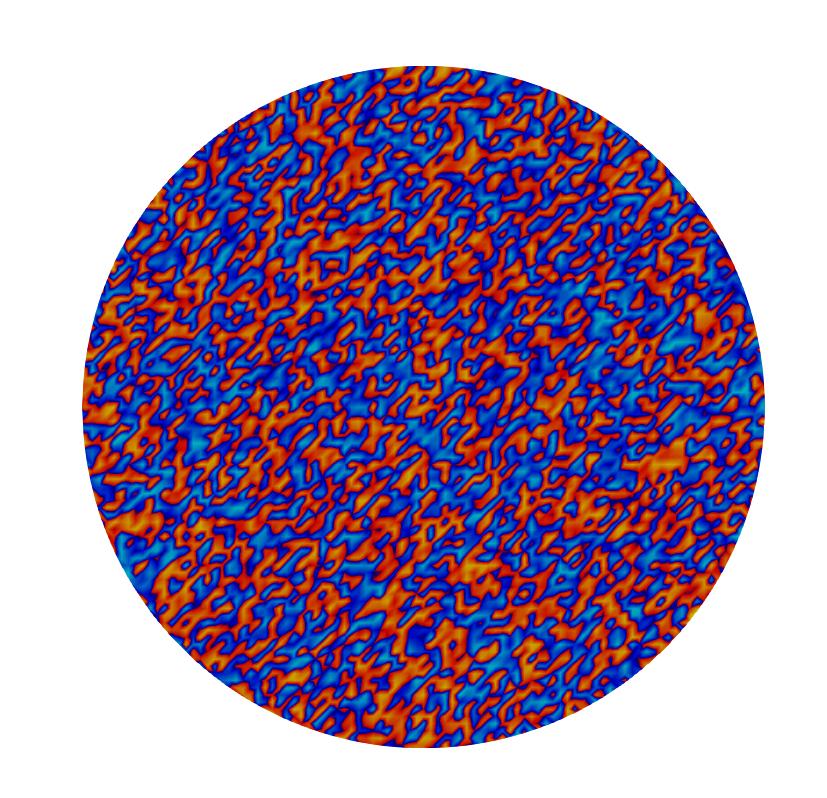
\includegraphics[width=0.3\textwidth]{results/illustration/c0.png}
    }\hfill
    \subfloat[$t=2\tau$]{\label{sub:fig:ill_c2}
        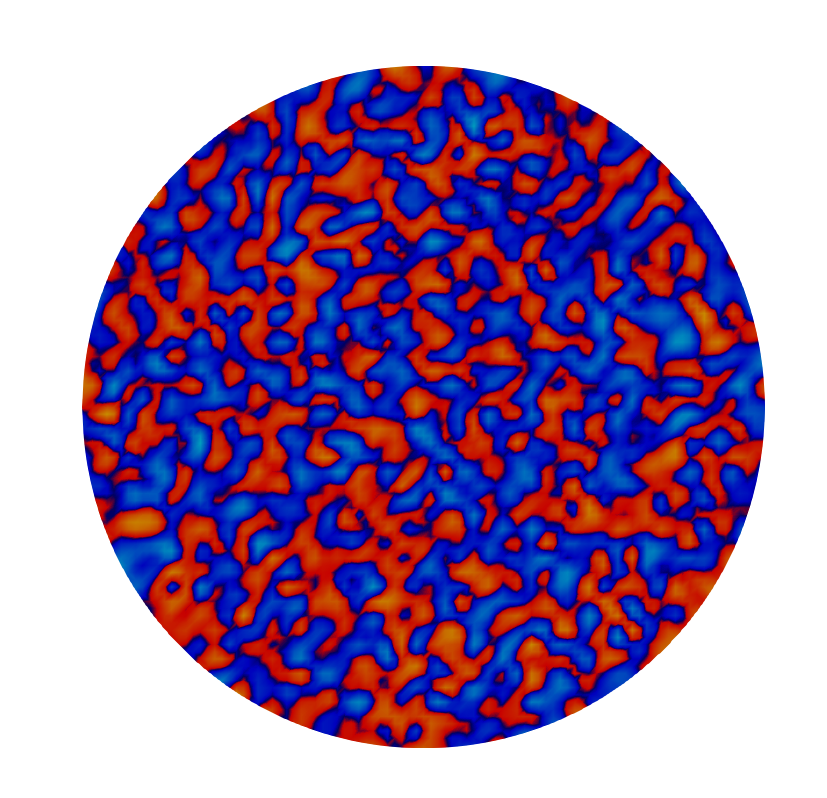
\includegraphics[width=0.3\textwidth]{results/illustration/c2.png}
    }\hfill
    \subfloat[$t=10\tau$]{\label{sub:fig:ill_c10}
        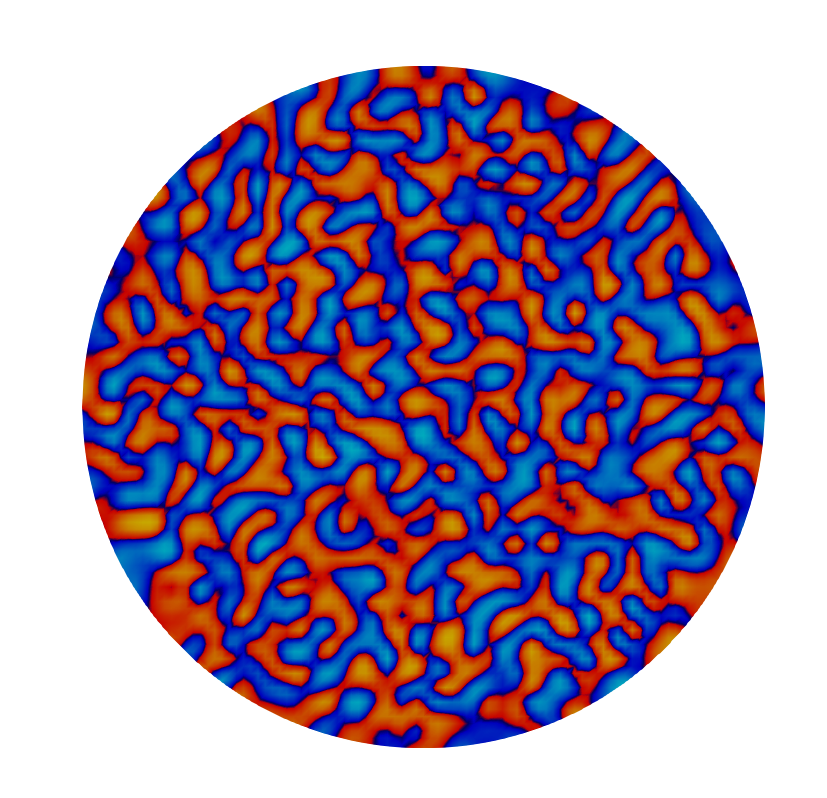
\includegraphics[width=0.3\textwidth]{results/illustration/c10.png}
    }
    \vspace{10pt}
    \subfloat[t=50$\tau$]{\label{sub:fig:ill_c50}
        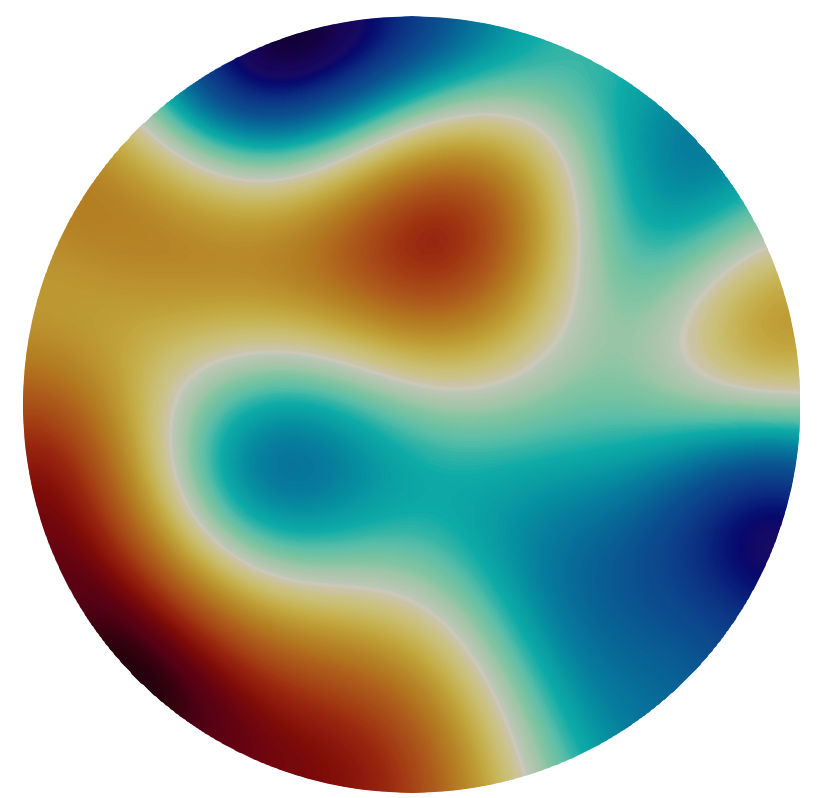
\includegraphics[width=0.3\textwidth]{results/illustration/c50.png}
    }\hfill
    \subfloat[$t=200\tau$]{\label{sub:fig:ill_c200}
        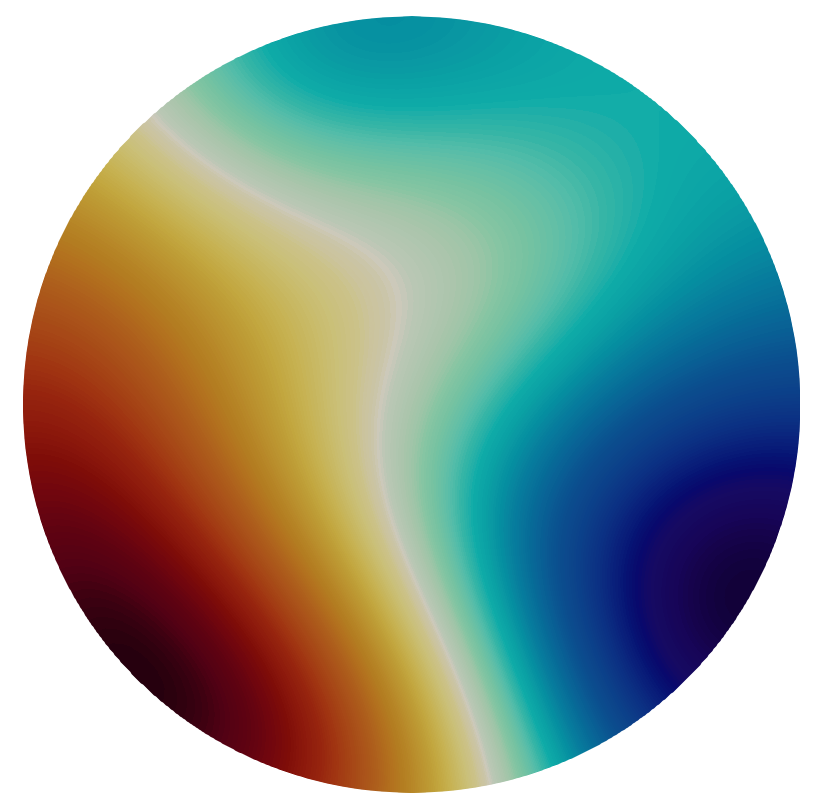
\includegraphics[width=0.3\textwidth]{results/illustration/c200.png}
    }\hfill
    \subfloat[$t=1000\tau$]{\label{sub:fig:ill_c1000}
        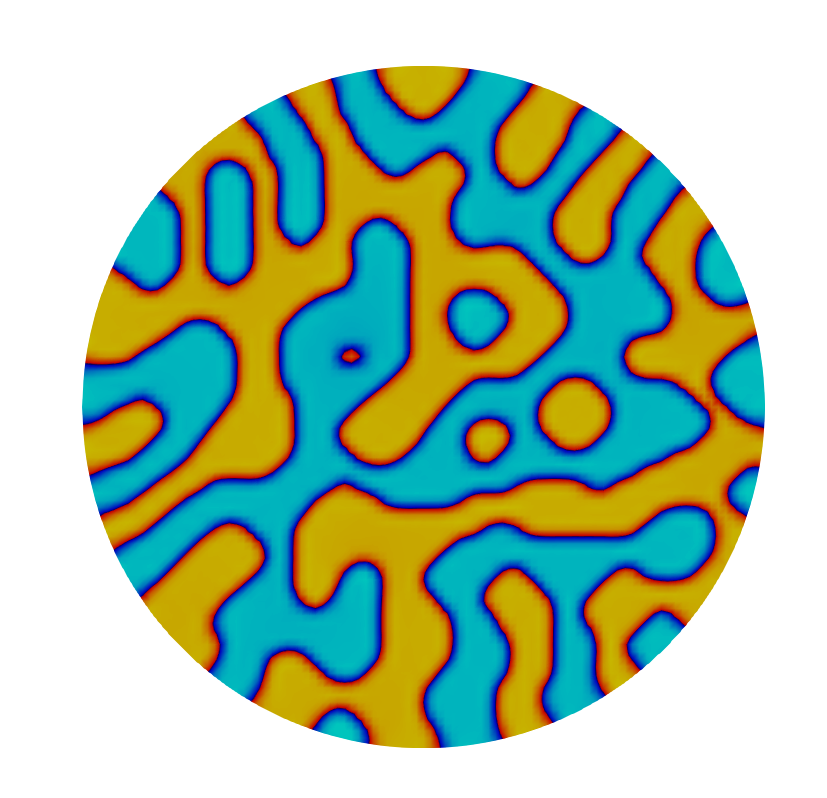
\includegraphics[width=0.3\textwidth]{results/illustration/c1000.png}
    }
    \caption{Overall caption for the first set of illustrations.}
\end{figure}

\begin{figure}[h!]
    \centering
    \subfloat[$t=0\tau$]{\label{sub:fig:ill_f0}
        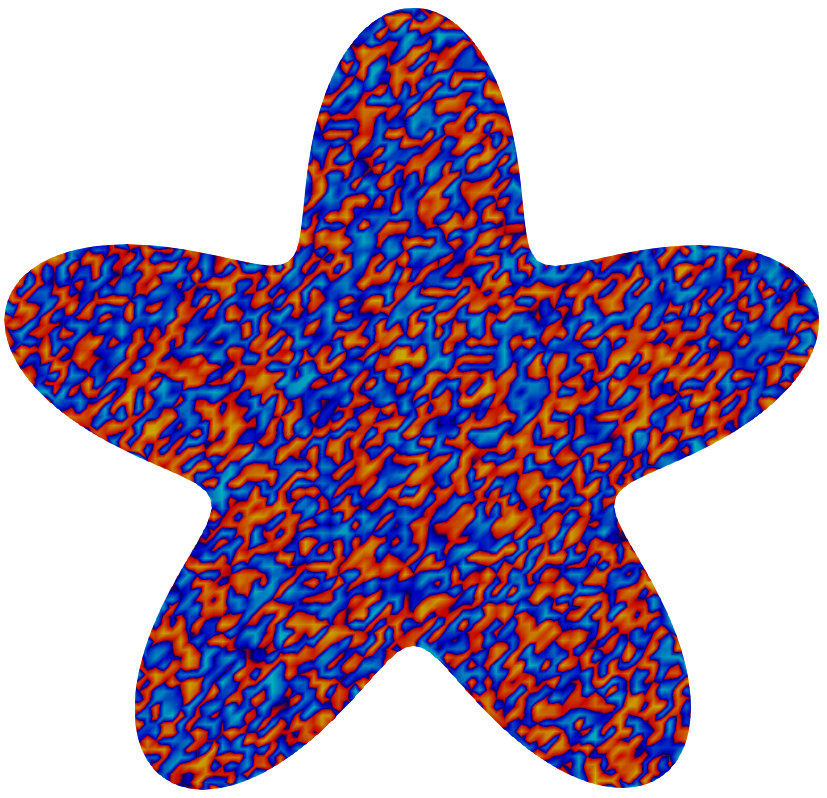
\includegraphics[width=0.3\textwidth]{results/illustration/f0.png}
    }\hfill
    \subfloat[$t=2\tau$]{\label{sub:fig:ill_f2}
        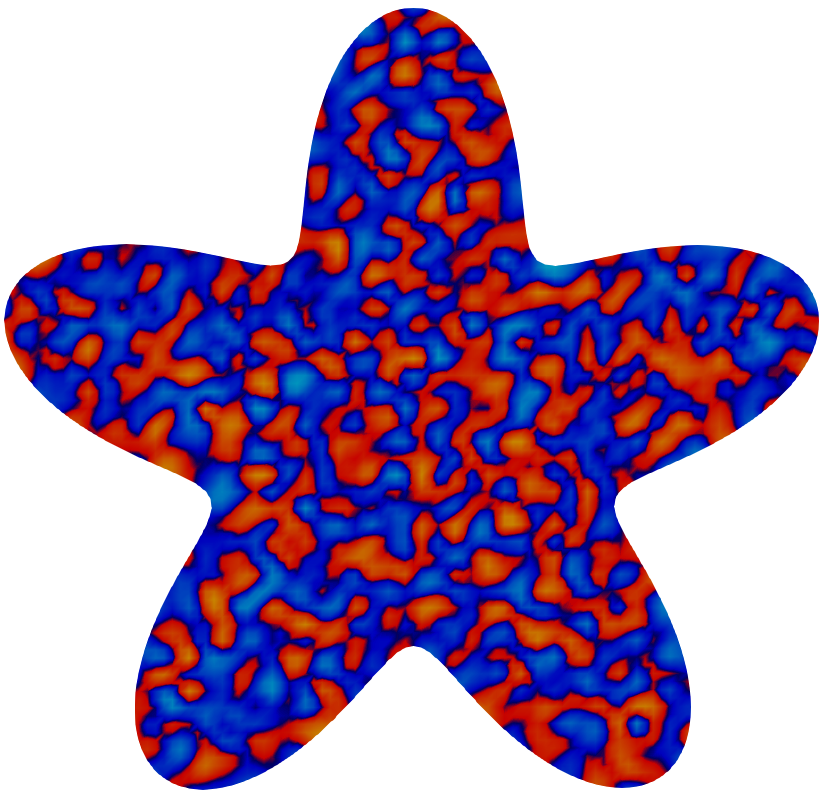
\includegraphics[width=0.3\textwidth]{results/illustration/f2.png}
    }\hfill
    \subfloat[$t=10\tau$]{\label{sub:fig:ill_f10}
        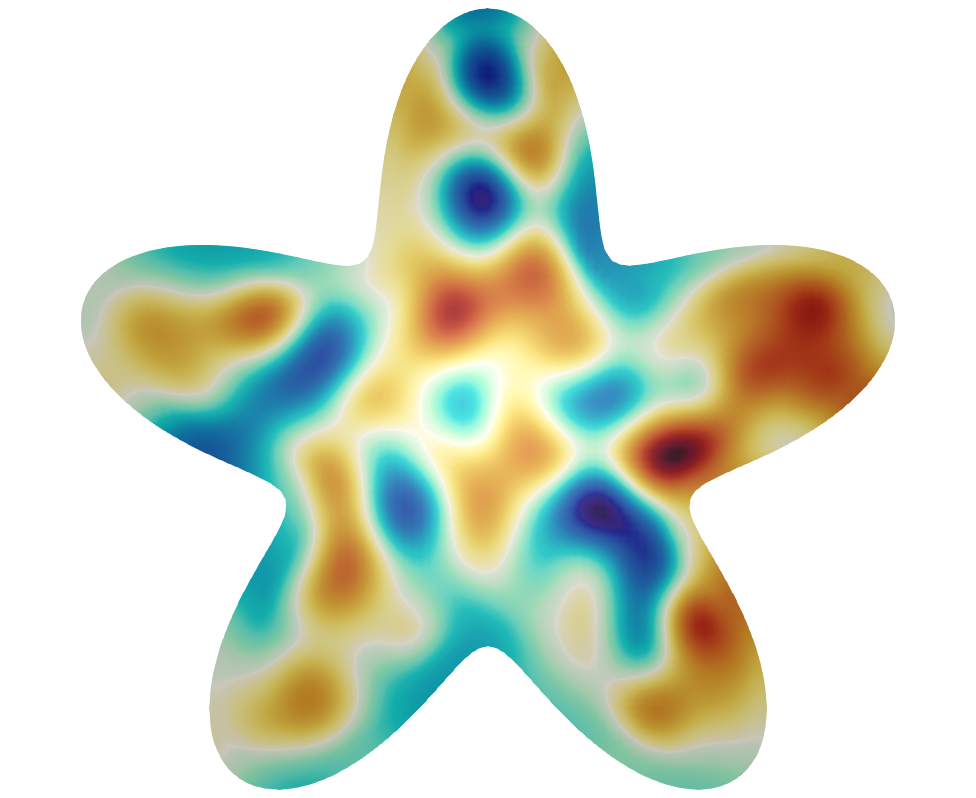
\includegraphics[width=0.3\textwidth]{results/illustration/f10.png}
    }
    \vspace{10pt}
    \subfloat[$t=50\tau$]{\label{sub:fig:ill_f50}
        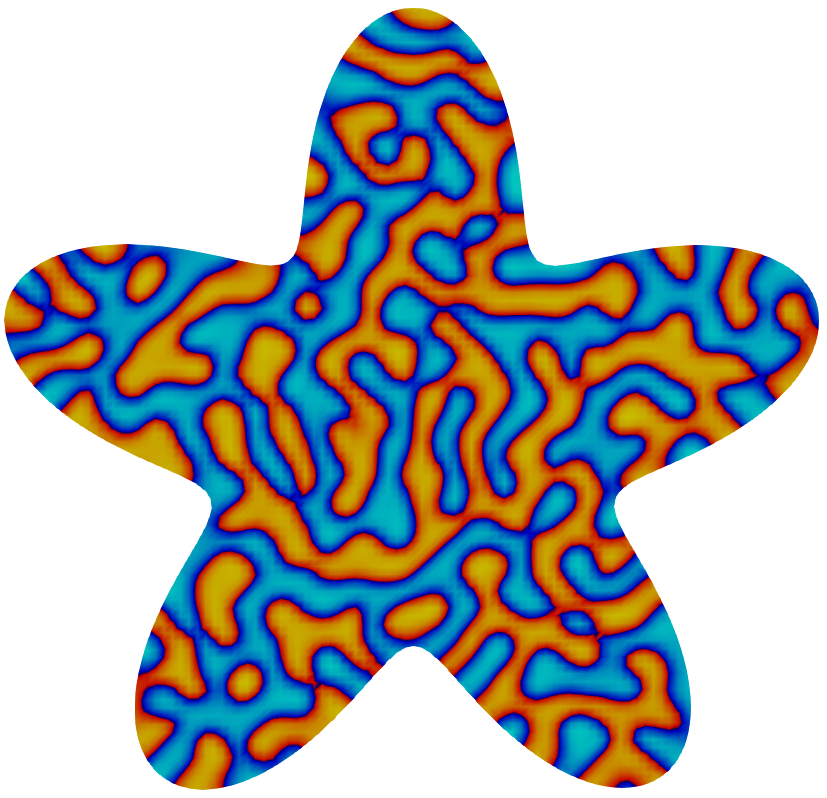
\includegraphics[width=0.3\textwidth]{results/illustration/f50.png}
    }\hfill
    \subfloat[$t=200\tau$]{\label{sub:fig:ill_f200}
        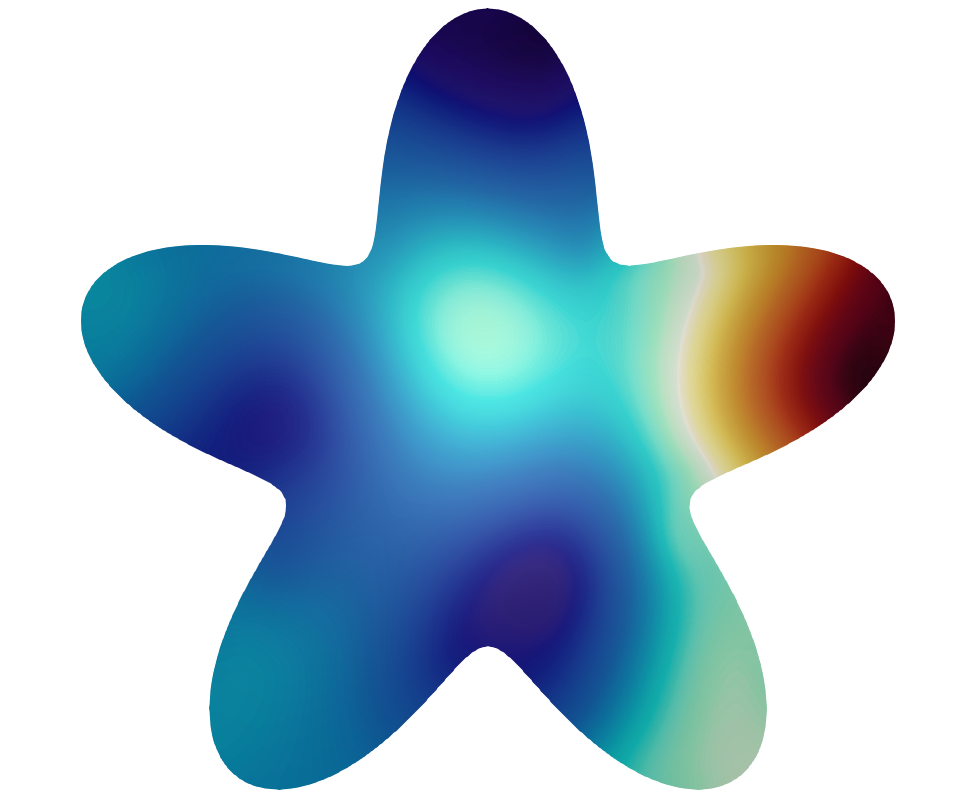
\includegraphics[width=0.3\textwidth]{results/illustration/f200.png}
    }\hfill
    \subfloat[$t=1000\tau$]{\label{sub:fig:ill_f1000}
        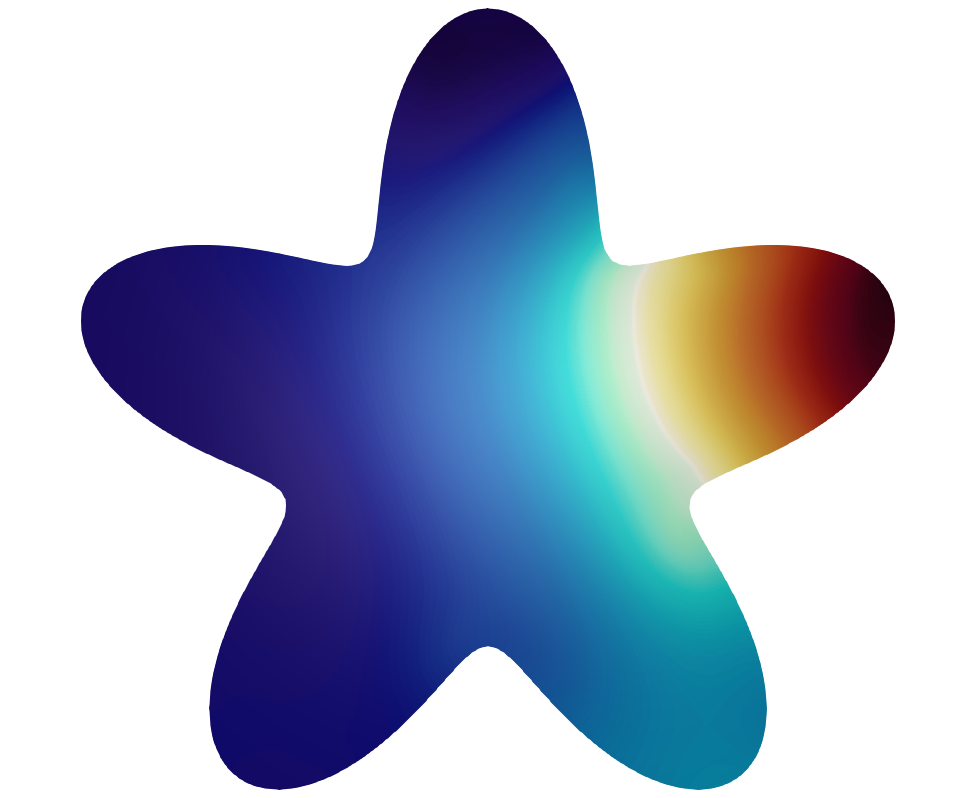
\includegraphics[width=0.3\textwidth]{results/illustration/f1000.png}
    }
\end{figure}
